\section{Performance}

The performance of the CLAS12 simulations is measured by comparing the predicted background rates from beam interactions
with the target with the actual experiment rates. The banchmarks are also quantified for each detector geometry and digitization routine.

\subsection{Comparison of rates with data}
On December 17 2017, the nominal luminosity of $10^{35} s{-1}cm{-2}$
(75 nA on a 5 cm liquid hydrogen target) was achieved in CLAS12.
The rates in various detectors were measured.

The Drift Chamber occupancy was compared for both FTon and FTOff configurations. The integrated occupancy
in region 1, 2 and 3 are summarized in tables \ref{tab:ftOnComparison} and \ref{tab:ftOffComparison}. The
time window of the experiment at the time was different than what was in the simulation, so the data has been scaled
accordingly. The predicted rates agree quite well with the measured ones. The occupancy distribution in the different layers
and wires also show good agreement between simulation and experiment, see \F{ftOnComparison} and  \F{ftOffComparison}.

\begin{table}[h]
	\begin{center}
		\begin{tabular}{| c | c | c |}
			Region & Data (rescaled) &  GEMC \\
			\hline
			1 &  $2.8\%$  & $2.68\%$ \\
			2 &  $0.6\%$  & $0.76\%$ \\
			3 &  $1.5\%$  & $1.18\%$ \\
		\end{tabular}
	\end{center}
	\caption{Drift Chambers rates comparison between simulation and real data for the FT On configuration}\label{tab:ftOnComparison}
\end{table}

\begin{table}[h]
	\begin{center}
		\begin{tabular}{| c | c | c |}
			Region & Data (rescaled) &  GEMC \\
			\hline
			1 &  $1.7\%$  & $1.12\%$ \\
			2 &  $0.3\%$  & $0.44\%$ \\
			3 &  $0.9\%$  & $0.73\%$ \\
		\end{tabular}
	\end{center}
	\caption{Drift Chambers rates comparison between simulation and real data for the FT Off configuration}\label{tab:ftOffComparison}
\end{table}


\begin{figure}
	\centering
	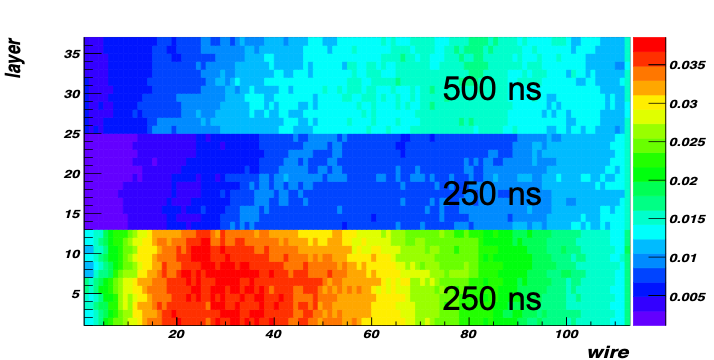
\includegraphics[width=0.95\columnwidth,keepaspectratio]{img/ftOnGemcDCRates.png}
	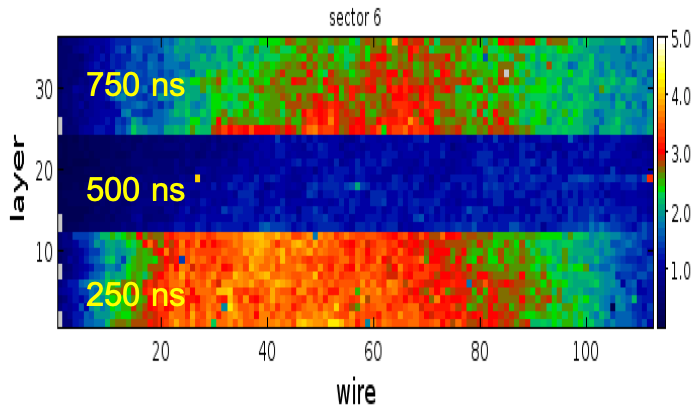
\includegraphics[width=0.95\columnwidth,keepaspectratio]{img/ftOnDataDCRates.png}
	\caption{Distribution of background events in the Drift Chamber region 1 for the FT On configuration.
             Top: gemc. Bottom: data.}
	\label{fig:ftOnComparison}
\end{figure}


\begin{figure}
	\centering
	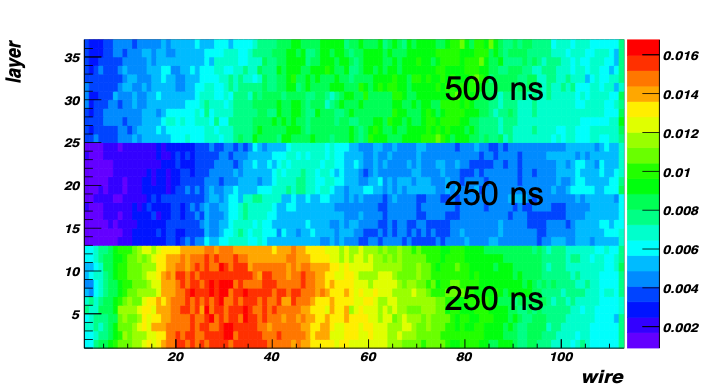
\includegraphics[width=0.95\columnwidth,keepaspectratio]{img/ftOffGemcDCRates.png}
	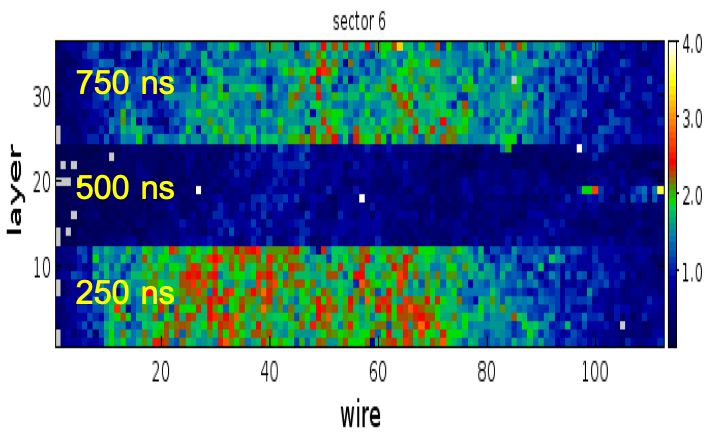
\includegraphics[width=0.95\columnwidth,keepaspectratio]{img/ftOffDataDCRates.png}
	\caption{Distribution of background events in the Drift Chamber region 1 for the FT Off configuration.
             Top: gemc. Bottom: data.}
	\label{fig:ftOffComparison}
\end{figure}

Simlar agreements were found in rates in other CLAS12 detectors: HTCC, EC and PCAL, FTOF and FT.

\subsection{Benchmarks}

The event rate has been measured in a single core for single and multiple tracks. The numbers reported here
refer to averages over several 2017 laptop and desktops and farm nodes.

The full CLAS12 geometry has been used, with Range Kutta field integration algorithm
and linear interpolation for both solenoid and torus fields.

Single meson tracks in the forward region are simulated with an event rate of about 10 Hz.
Electron rates are about half as fast due to shower in the EC and PCAL calorimeters and
Cherenkov photons production in both HTCC and LTCC, for an average of 5 Hz.

A quantitative study of the event rate for 3 particles (2 in the forward detector, one in the central)
details the time spend in each detector geometry and digitization and in each magnetic field.
The particles generated are:

\begin{itemize}
	\item one 7 GeV electron between 15 and 25 degrees in theta.
	\item one 2 GeV gamma between 15 and 25 degrees in theta
	\item one 2 GeV proton at 90 degrees in theta
\end{itemize}

The results are shown in table \ref{tab:benchmarks}. The final rate for the 3 particles in the
complete CLAS12 setup is 1.9 Hz.

\begin{table}[h]
	\begin{center}
		\begin{tabular}{ c | c | c | c }
			 & Rate (Hz) &  ms / event &  $\%$ of total\\
			\hline
Target   &  555.8  &   1.8   & 0.3  \\
SVT      &  365.9  &   0.9   & 0.2  \\
MM       &  48.9   &   17.7  & 3.4  \\
CTOF     &  48.7   &   0.1   & 0.0  \\
Solenoid &  15.8   &   42.8  & 8.1  \\
HTCC     &  11.5   &   24.0  & 4.5  \\
FT       &  11.2   &   2.4   & 0.4  \\
DC       &  8.1    &   33.2  & 6.3  \\
LTCC     &  6.5    &   30.6  & 5.8  \\
FTOF     &  6.1    &   9.6   & 1.8  \\
PCAL     &  2.8    &   196.2 & 37.1 \\
EC       &  2.0    &   134.5 & 25.4 \\
Torus    &  1.9    &   34.7  & 6.6  \\
		\end{tabular}
	\end{center}
	\caption{Drift Chambers rates comparison between simulation and real data for the FT Off configuration}\label{tab:benchmarks}
\end{table}

Background rate can be estimated by setting a time window to define the time length of one event, and
generating a number of electrons proportional to the proposed beam current. For the nominal luminosity of $10^{35} s{-1}cm{-2}$
this correspond to 124,000 electrons in a 250 ns time window. In this case the time to complete one event varies
between one and two minutes depending on CPU flavor and available memory.

































